\begin{figure}
	\centering
	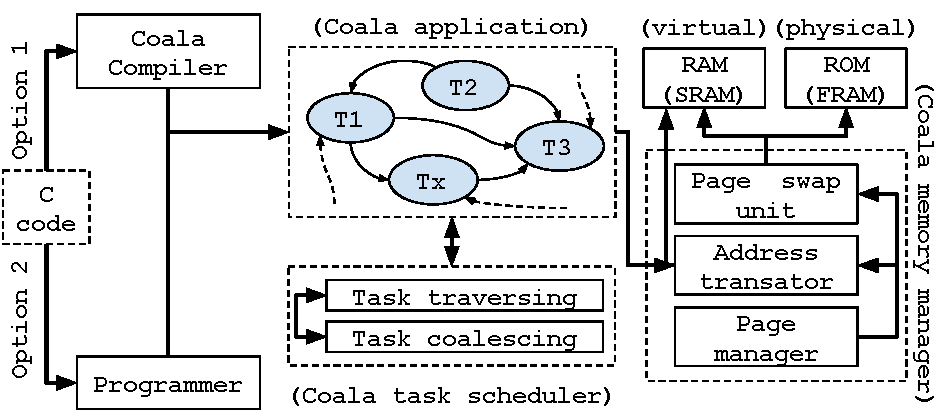
\includegraphics[width=\columnwidth]{figures/viper_block_diagram.pdf}
	\caption{\sys top-level view.}
	\label{fig:system_overview}
\end{figure}

\sys is a new programming and execution model for intermittent computing on
energy-harvesting devices.  \sys addresses the challenges motivated in
Section~\ref{sec:background} to make task-based intermittent programs {\em
efficient}, {\em flexible}, and {\em programmable}.  \sys accomplishes this
goal with a constellation of a new programming model, compiler, and run time
software system support.  Figure~\ref{fig:system_overview} shows a block
diagram overview of \sys.

To use \sys, a programmer first writes plain, imperative C code.  The
programmer then has an option to {\em manually} or {\em automatically}
translate their program into code for \sys's task-based programming  model.  We
describe the programming primitives involved in either translation in
Section~\ref{sec:overview:programming}.
%
To manually translate the programmer decomposes the program into tasks, and
annotates memory accesses that manipulate data shared by multiple tasks.  To
automatically translate, the programmer simply uses \sys's compiler (described
in Section~\ref{sec:compiler}), which decomposes a program into tasks and
annotates accesses to task-shared data. 
%
After translating to task-based code and compiling, the programmer has an
executable \sys binary.  

When the binary executes, \sys's runtime support affects its execution through
its {\em virtualizing memory manager} and through its {\em coalescing task
scheduler}.
%
The \sys binary executes its tasks correctly and with consistent memory state
due to \sys's virtual memory mechanism.  Relying on programmer or compiler
annotation of accesses to memory locations that might be shared beetween tasks,
\sys's memory virtualization {\em pages} these data to SRAM from FRAM as they
are needed.  Tasks operate, accessing SRAM only, demand-paging data in to
accomodate an SRAM smaller than FRAM.  When a task completes, \sys commits
modified, paged data back to its original FRAM location atomically ensuring
that subsequent tasks page in correct memory state. 

\sys runs a lightweight task scheduler that uses {\em task coalescing} to make
\sys's statically defined tasks efficiently use available energy.  By default,
tasks run in sequence and each task commits as it completes, potentially
incurring unnecessary overhead for commits between consecutive, non-failing
tasks.  \sys dynamically coalesces consecutive tasks by deferring the commit of
an earlier task until the completion of a later task.  \sys's memory management
mechanism facilitates coalescing because \sys can defer an earlier task's
commit by simply buffering modified, paged data as the later task executes.
After coalescing a sequence of tasks, \sys commits all tasks' updates to FRAM,
together, combining tasks updates to the same pages and minimizing the commit
overhead.


\subsection{Programming Model}
\label{sec:overview_programming_model}

\begin{table}
	\centering
	\footnotesize
	\begin{tabular}{|c|c|}
		\hline
		Keyword & Description\\
		\hline\hline
		\texttt{RP} & Read-protected variable\\
		\texttt{WP} & Write-protected variable\\
		\texttt{\_\_task\_\_ foo(){...}} & Task declaration\\
		\texttt{addTask()} & Build internal data structure for executor \\
		\texttt{run\_tasks()} & Task executor \\ %scheduler
		\texttt{next\_task()} & Transition to a new task\\
		%\texttt{PageFault()} & --- \\
		%\texttt{P()} & ---\\
		\hline
	\end{tabular}
\caption{Summary of \sys syntax: top---user-specific variables}
\label{tab:viper_syntax}
\end{table}
